\documentclass[handout]{beamer} % [handout] para imprimir eliminando transiciones

%\usefonttheme[onlymath]{serif}
%\usepackage{fontspec}
%\defaultfontfeatures{Mapping=tex-text}
%\setsansfont[Ligatures={Common}]{Futura}
%\setmonofont[Scale=0.8]{Monaco} 

\usepackage{beamerthemesplit}
\usepackage[utf8]{inputenc}
\usepackage[spanish]{babel}
\mode<presentation>
\usetheme{default}
\usecolortheme{dolphin}
\usepackage{alltt}                                    % \begin{alltt}
\usepackage{amssymb}                                  % mathematical symbols
\usepackage{comment}
\usepackage{url}
\usepackage{tabto}                                    % \tabto
\usepackage{tikz}
\usetikzlibrary{automata}
\usetikzlibrary{positioning}
\usetikzlibrary{calc}

\usepackage{verbatim}                                 % comentarios

\title{Lenguajes de Programación}                     %[titulo corto]
\author{Fabián Riquelme Csori}                        %[nombre corto]
\date{2017}                                           %[fecha corta]
\institute{Universidad de Valparaíso}                 %[instituto corto]

\newcommand{\HRule}{\rule{\linewidth}{0.2mm}\\[1ex]}
\newcommand{\blue}[1]{\textcolor{blue}{#1}}
\newcommand{\red}[1]{\textcolor{red}{#1}}
\newcommand{\redb}[1]{{\color{red!70!black}{#1}}}
\newcommand{\green}[1]{{\color{green!70!black}{#1}}}
\newcommand{\gray}[1]{{\color{gray!50!white}{#1}}}
\newcommand{\yell}[1]{{\color{yellow!70!black}{#1}}}
\newcommand{\lQ}{\mbox{``}}
\newcommand{\rQ}{\mbox{''}}
% \alert{texto destacado en rojo}
% \color{green} Color en verde
% \structure{texto en lila}


\begin{document}

%\begin{frame}%[plain]
%  \titlepage
%\end{frame}
%
% [opciones]:
% plain: oculta barra de navegacion, deja + espacio para contenido
% fragile: usar comandos como verbatim
% b,c,t: alineacion vertical
% label=nombre_etiqueta
% allowframebreaks: divide contenido en varios frames si es demasiado largo
% shrink: para escribir mucho texto en una transparencia, reduciendo tamano de fuente

%%%%%%%%%% PORTADA %%%%%%%%%%
\begin{frame}[plain]
  \begin{figure}[h]
    \begin{minipage}{0.3\textwidth}
    
\includegraphics[width=.9\textwidth]{./image/logo-UV.png}
    \end{minipage}
    \begin{minipage}{0.65\textwidth}
     $~$\\[3.6ex]
     \footnotesize{Escuela de Ingeniería Civil Informática}\\
     \footnotesize{Facultad de Ingeniería}
    \end{minipage}
  \end{figure}
  \begin{center}
    \vspace{1ex}
    \HRule
    \Large{Lenguajes de Programación}\\{\small Capítulo IX: Lenguajes de Scripting}\\[-1ex]
    \HRule\vspace{1ex}
    \large{Fabián Riquelme Csori}\\[.5ex]\footnotesize{fabian.riquelme@uv.cl}\\[6ex] {\tiny 2017-II}\\[6ex]
  \end{center}
\end{frame}

%%%%%%%%%% INDEX %%%%%%%%%%
\begin{frame}
 \frametitle{Index}
 \scriptsize 			% reducir tamano de letra
 \tableofcontents		%[pausesections]
\end{frame}

%%%%%%%%%%% ACTUAL INDEX %%%%%%%%%%
%\AtBeginSection[] %generar indice automaticamente
%{
%\begin{frame}<beamer>%[plain]
% \frametitle{Index}
% \framesubtitle{subtitulo}
% \scriptsize
% \tableofcontents[currentsection, currentsubsection]
%\end{frame}
%}

%==============================
\section{Lenguajes de Scripting}

%------------------------------
\subsection{Introducción}

\begin{frame}{Introducción}
  \begin{itemize}
    \item<1-> Los lenguajes de programación tradicionales enfrentan problemas computacionales de manera autónoma: reciben un input y generan un output.
    \item<2-> Pero la mayoría de problemas del mundo real involucran múltiples tareas o pasos.
    \item<3-> Ejemplo:
    \begin{itemize}
        \item Un sistema almacena una lista de números en un archivo txt (un número por línea).
        \item Cada número debe enviarse a una BD como un parámetro para una consulta SQL.
        \item Cada consulta retorna un string que representa un comando que debe ejecutar el sistema operativo.
    \end{itemize}
    \item<3-> Este problema puede tratarse de múltiples maneras...
  \end{itemize}
\end{frame}

\begin{frame}{Opción 1: usar un lenguaje tradicional (como Java)}

  {\small
  public int getNumFromFile () \{\\
  $~~~$...\\
  $~~~$return Integer.parseInt(BufferedReader.readLine());\\
  \}\\[1.5ex]
  public String executeSQL ( int c ) \{
  $~~~$...\\
  $~~~$return SQL(``select command from table where command = ''+c);\\
  \}\\[1.5ex]
  public void executeCommand ( String command ) \{\\
  $~~~$...\\
  $~~~$Runtime.exec(command);\\
  \}}
\end{frame}

\begin{frame}{Opción 1 (cont.)}
  \begin{itemize}
    \item Los lenguajes como Java enfatizan aspectos como \blue{eficiencia}, \blue{portabilidad} y \blue{mantenibilidad}.
    \item Sus sistemas de tipos (de datos) se basan en conceptos a nivel de hardware.
    \begin{itemize}
        \item Enteros de tamaño fijo, puntos flotantes, carácteres y arreglos.
    \end{itemize}
  \end{itemize}
\end{frame}

\begin{frame}{Opción 2: usar pequeño un script bash}

  {\small
  read –r  var1 $<$ commands.txt\\
  while \$var1 –ne ``''\\
  $~~~~$do\\
  $~~~~~~~~$echo ``select command from table where\\
  $~~~~~~~~~~~~~~~~~~~~~~~~~~~~~~~~~~~~~~~~~~~~$command =''\$var1 $>$ query.txt\\
  $~~~~~~~~$mysql $<$ query.txt $>$ command\\
  $~~~~~~~~$read –r var2 $<$ command\\
  $~~~~~~~~$exec \$var2\\
  $~~~~~~~~$read –r var1 $<$ commands.txt\\
  $~~~~$done}
  \vspace{4ex}
  
  \begin{flushright}
    ...de menos de 10 líneas!
  \end{flushright}
\end{frame}

\begin{frame}{Opción 2 (cont.)}
  \begin{itemize}
    \item Los lenguajes de scripting enfatizan aspectos como \blue{flexibilidad}, \blue{desarrollo rápido} ($\neq$ ágil) y \blue{chequeo dinámico}.
    \item Sus sistemas de tipos se basan en conceptos de \blue{muy alto nivel}.
    \begin{itemize}
        \item Tablas, patrones, listas y archivos.
    \end{itemize}
  \end{itemize}
\end{frame}

%------------------------------
\subsection{Características}

\begin{frame}{Lenguajes de scripting}

  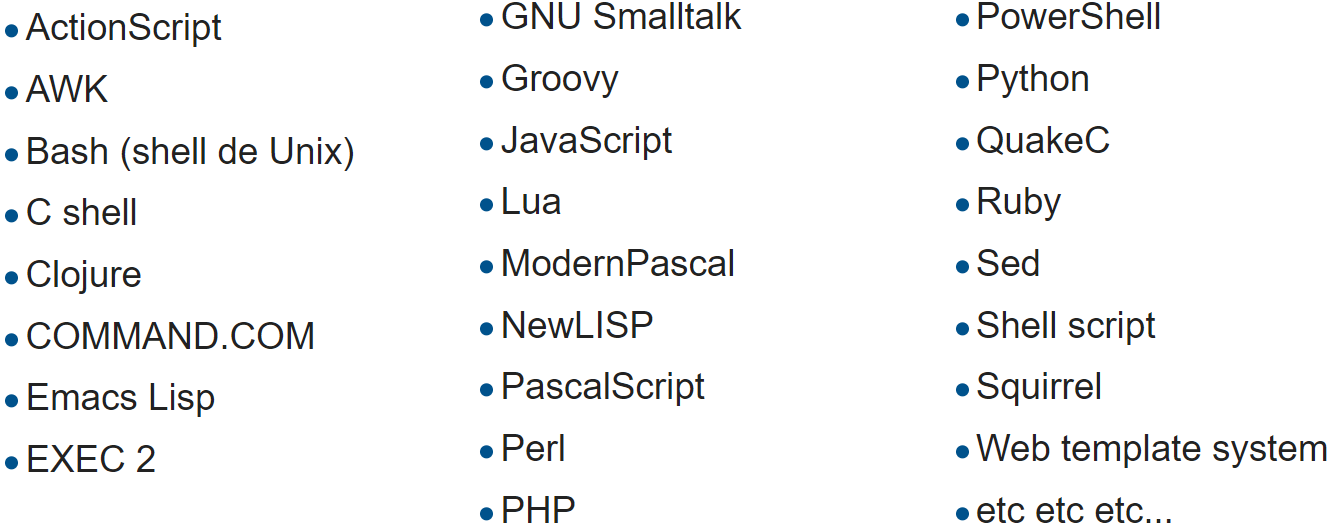
\includegraphics[width=\textwidth]{./image/cap9/lenguajes-scripting.png}
\end{frame}

\begin{frame}{Lenguajes de scripting}
  \begin{itemize}
    \item<1-> Los lenguajes de scripting son muy variados
    \item<2-> Clasificación por dominio de uso:
    \begin{itemize}
        \item Lenguajes de dominio específico: servicios web, videojuegos, GUI scripting, etc.
        \item Lenguajes de propósito general. \textbf{\blue{Glue languages}}: Perl, Python, Ruby, Scheme, sh, etc.
    \end{itemize}
    \item<3-> Dos tipos de ancestros:
    \begin{itemize}
        \item Intérpretes de comandos o ``shells'': terminal en modo batch.\\Ej: sh y csh de Unix, archivos .bat de MS-DOS.
        \item Lenguajes diseñados para procesamiento de texto y generación de reportes.\\
        Ej: \blue{sed} y \blue{awk}, en los que se basó \blue{Perl}.
    \end{itemize}
  \end{itemize}
\end{frame}

\begin{frame}{Scripting en desarrollo web}
  \begin{itemize}
    \item<1-> Perl (n.1987) se adoptó en la primera mitad de los 90's para trabajar en procesamiento del lado del servidor.
    \item<2-> La gran cantidad de scripts necesarios llevaron al desarrollo de un lenguaje independiente: \blue{PHP} (n.1995).
    \item<3-> Como alternativas a PHP, luego aparecieron Java\blue{Script} y VB\blue{Script} (Windows), Apple\blue{Script} (Mac).
    \item<4-> Los scripts pueden ser embebidos dentro del HTML.
    \item<5-> La idea es buscar la independencia de plataformas y compatibilidad con navegadores web de clientes.
    \item<6-> Sentencias sencillas permiten ejecutar numerosas instrucciones de máquina.
  \end{itemize}
\end{frame}

\begin{frame}{Características genéricas}
  \begin{itemize}
    \item Suelen ser \blue{lenguajes interpretados} (no compilados).
    \item Mayormente \blue{imperativos} (no orientados a objeto).
    \item Para uso interactivo y modo bash.
    \item Ausencia de declaraciones; reglas simples de \blue{scoping}.
    \item Tipos de datos de alto nivel.
    \item Administración de memoria automática (no hay manejo de punteros como en C/C++).
  \end{itemize}
\end{frame}

\begin{frame}{Ventajas y desventajas}
  \pause
  \begin{block}{Ventajas}
  \begin{itemize}
    \item Economía y expresividad.
    \item Fácil acceso a otros programas.
    \item Potentes patrones de {\em matching}.
    \item Sintaxis sencilla, flexible y dinámica:\\[1.5ex]
    {\scriptsize
    \red{public static void main(String args[])\{\\
	$~~$System.out.println(``Hola mundo'');\\
    \}} vs.\\
    \green{print ``Hola mundo''}}
  \end{itemize}
  \end{block}
  \pause
  \begin{block}{Desventajas}
  \begin{itemize}
      \item Más lentos que lenguajes compilados (el código se interpreta en tiempo de ejecución).
  \end{itemize}
  \end{block}
\end{frame}

%==============================
\section{Data frames}

%------------------------------
\subsection{Generalidades}

\begin{frame}{Data frames}
  \begin{itemize}
    \item Un \blue{data frame} puede entenderse como una estructura de datos que soporta {\em data sets} o conjuntos de datos tabulados.
  \end{itemize}
  \begin{center}
      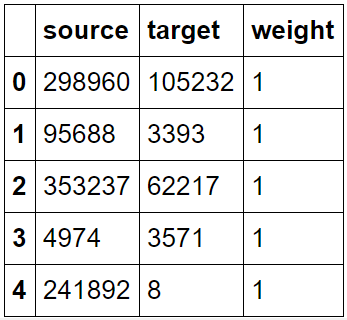
\includegraphics[width=.4\textwidth]{./image/cap9/dataframe.png}
  \end{center}
  \begin{itemize}
      \item<2-> Cada columna posee un tipo de datos homogeneo.
      \item<3-> La fila y columna en negritas se consideran \blue{metadatos}.
  \end{itemize}
\end{frame}

\begin{frame}{Aplicaciones}
  \begin{itemize}
    \item<1-> Los data frames vienen del mundo de los software estadísticos y sus evoluciones.
    \begin{center}
      
\includegraphics[width=.8\textwidth]{./image/cap9/tecnologias.png}
    \end{center}
    \item<2-> Desde R vinieron a reemplazar a las matrices de Matlab.
    \item<3-> Su gracia es que proveen muchas funciones para el manejo de datos que facilitan las operaciones matemáticas de validación, selección, normalización, adición, etc.
  \end{itemize}
\end{frame}

\begin{frame}{Poder de los dataframes}
  \begin{itemize}
    \item Los dataframes no son simples tablas de datos como plantillas Excel o bases de datos relacionales.
    \item Permiten lidiar con dos problemas especialmente recurrentes en big data:
    \begin{itemize}
        \item<2-> Violaciones a restricciones de integridad.
        \item<2-> Datos desconocidos o incompletos.
    \end{itemize}
  \end{itemize}
\end{frame}

%------------------------------
\subsection{Python: Pandas + Jupyter}

\begin{frame}{Trabajar con dataframes}
  \begin{itemize}
    \item Una manera bastante poderosa de trabajar con data frames es mediante Python:
    \begin{itemize}
        \item Con la librería \blue{Pandas}.
        \url{http://pandas.pydata.org/}
        \item Con \blue{Jupyter}, ambiente interactivo que permite trabajar con \blue{notebooks}: combinar código de ejecución, texto enriquecido, matemáticas, gráficos y otros. \url{https://jupyter.org/}
    \end{itemize}
    \item En lugar de Pandas podríamos trabajar con \blue{Spark}, que además favorece la escalabilidad por su capacidad para trabajar con sistemas distribuidos.
  \end{itemize}
\end{frame}

\begin{frame}{Trabajar con dataframes}
  \begin{itemize}
    \item Ayuda de instalación y primeros pasos:\\ \blue{\url{http://nikgrozev.com/2015/12/27/pandas-in-jupyter-quickstart-and-useful-snippets/}}
    \item Ejemplos de notebooks de uso real:\\ \blue{\url{https://github.com/GCantergiani/centrality-measure-lth-model/tree/master/notebooks}}
  \end{itemize}
\end{frame}

\begin{frame}{Ejercicios}
  \begin{itemize}
    \item Ver lecciones 9, 10 y 11 del curso intensivo de Roberto Muñoz (introducción, visualización y análisis con Pandas):\\ {\scriptsize \blue{\url{https://github.com/MetricLearning/intensivo_python}}}
    \item Reproducir la visualización de aeropuertos en el mundo.
    \item Modificar color de acuerdo con altitud. \blue{(bonus +1)}
    \item Visualizar \texttt{rutas.csv} como un grafo de rutas, cuyos nodos son los distintos países y las aristas tienen la forma (\texttt{Pais\_origen}, \texttt{Pais\_destino}). \blue{(bonus +2)}
  \end{itemize}
\end{frame}

%------------------------------

\begin{frame}
 \begin{block}{Bibliografía}
  \begin{itemize}
    \item Pratt, Terrence W. (1998). \textit{Lenguajes de programación: diseño e implementación}, Pearson Education.
    \item Sethi, Ravi (1992). \textit{Lenguajes de programación: conceptos y constructores}, Addison-Wesley Iberoamericana.
    \item Scott, Michael (2009). \textit{Programming Language Pragmatics}, Morgan Kaufman, 3ra ed.
  \end{itemize}
 \end{block}
 \begin{block}{Recursos}
  \begin{itemize}
    \item Wikipedia y Wikimedia Commons.
  \end{itemize}
 \end{block}
\end{frame}

\end{document}
